In task 1 we want to compute two equilibria for our system, define a reference curve between them and then compute the optimal transition to move from one equilibrium to another exploiting the Newton's$-$like algorithm for optimal control.

\section{Equilibrium Computation}

To compute the equilibria of the system, we set the derivatives of the system to zero:


\[
\begin{cases}
\begin{aligned}
&x_{5,t+1} - x_{5,t} = \frac{\delta}{m+M} \bigl[m L x_{7,t}^2 \sin(x_{3,t}) +\\
&\qquad - u_{1,t} \bigl(\sin(x_{4,0}) - \frac{m}{M} \sin(x_{3,t} - x_{4,t}) \cos(x_{3,t})\bigr)\bigr] = 0 \\
&x_{6,t+1} - x_{6,t} = \frac{\delta}{m+M} \bigl[(-m L x_{7,t}^2 \cos(x_{3,t}) +\\
&\qquad + u_{1,t} \bigl(\cos(x_{4,0}) + \frac{m}{M} \sin(x_{3,t} - x_{4,t}) \sin(x_{3,t})\bigr)\bigr) - g] = 0 \\
&x_{7,t+1} - x_{7,t} = \frac{\delta}{M L} [-u_{1,t} \sin(x_{3,t} - x_{4,t})] = 0 \\
&x_{8,t+1} - x_{8,t} = \frac{\delta}{J} l u_{2,t} = 0
\end{aligned}
\end{cases}
\]



Solving this system could lead to four possible configurations, but we will only consider the following case:
\[
\begin{cases}
x_{3,t} = 0\\
x_{4,t} = x_{3,t}\\
u_{1,t} = (M + m) g\\
u_{2,t} = 0
\end{cases}
\]

Note that this equilibrium point can represent either a stationary position or a constant velocity.

\section{Reference trajectory definition}

The planned path is made using the starting and ending equilibrium points. This path looks the same on both sides, with two long steady parts in between. Keep in mind that this reference trajectory is not a feasible trajectory for the system dynamics.

Here an example of reference trajectory.

\begin{figure}[h]
  \centering
  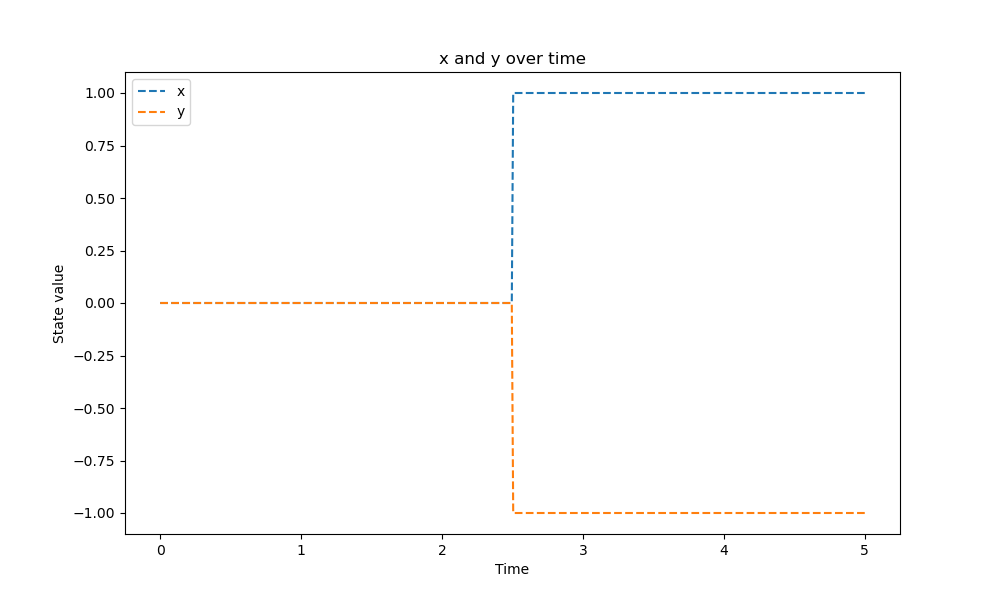
\includegraphics[width=0.9\textwidth]{pictures/x_y ref.png}\hfill\\
  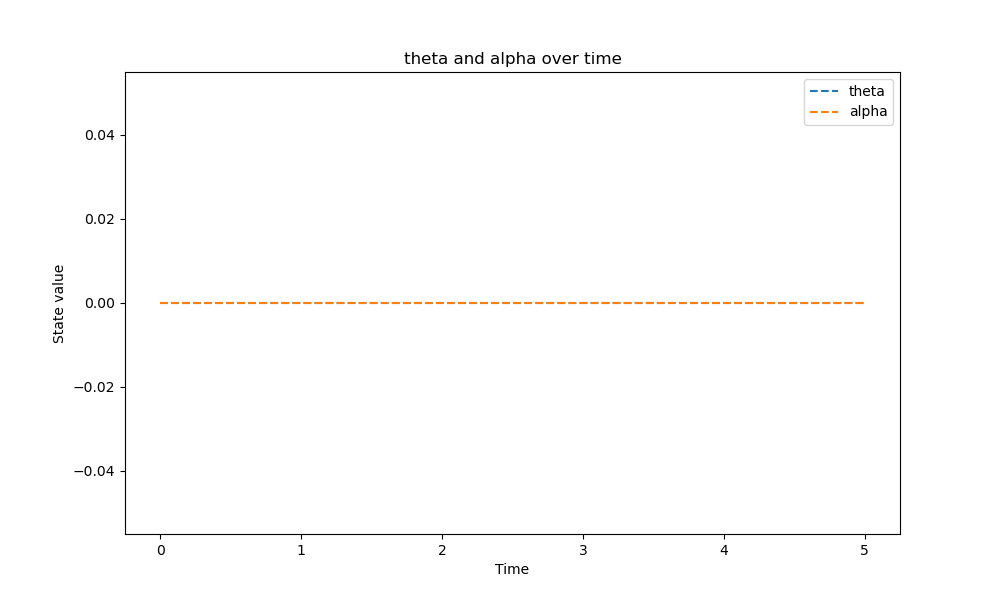
\includegraphics[width=0.9\textwidth]{pictures/theta_alpha ref.png}\hfill
  \caption{configuration reference over time.}
  \label{fig:Reference trajectory}
\end{figure}

\begin{figure}[H]
  \centering
  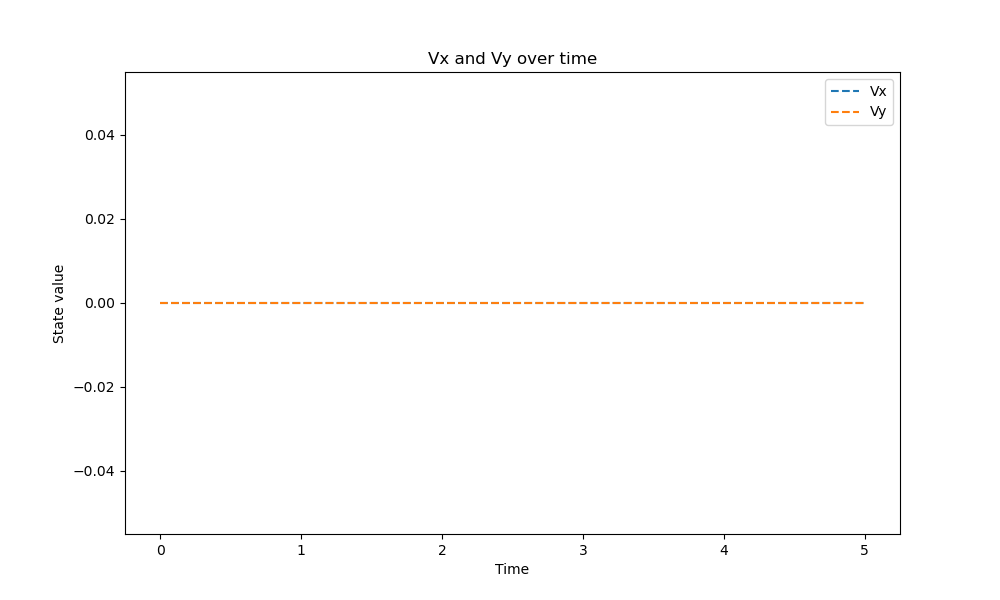
\includegraphics[width=0.85\textwidth]{pictures/Vx_vyreef.png}\hfill \\
  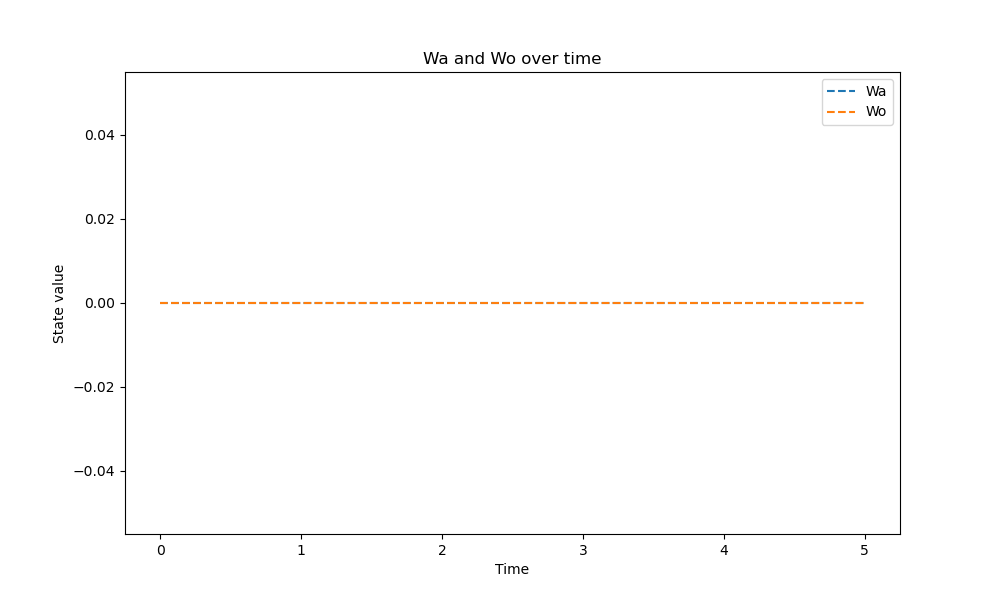
\includegraphics[width=0.85\textwidth]{pictures/wa wo ref.png}\hfill
  \caption{velocities reference over time.}
  \label{fig:Reference trajectory}
  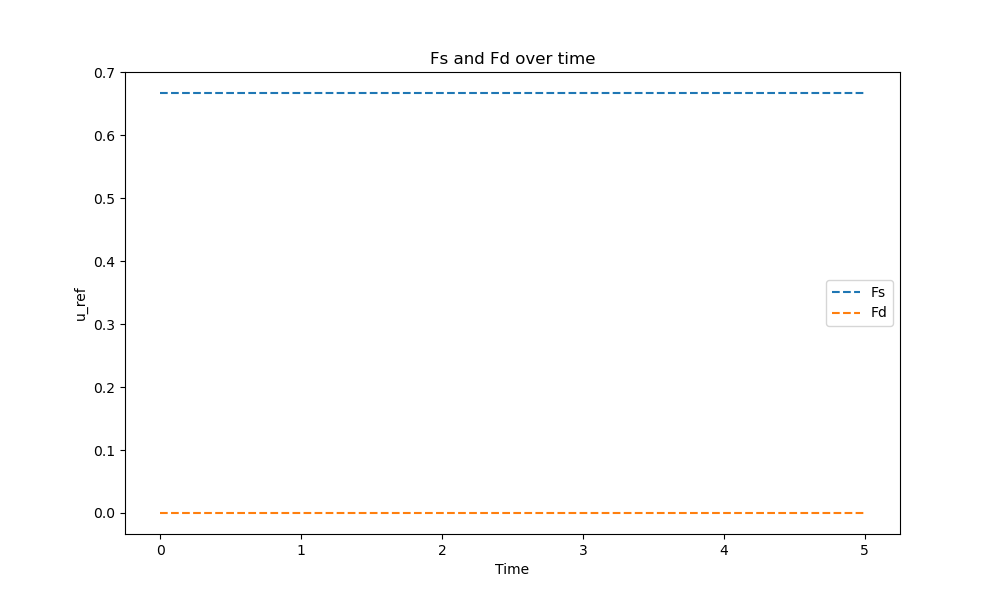
\includegraphics[width=0.85\textwidth]{pictures/Fs fd ref.png}
  \caption{Input reference over time.}
  \label{fig:Reference trajectory}
\end{figure}


\section{Linear Quadratic Regularization}
To solve the optimal control problem we implemented Linear Quadratic Regularization (LQR).
\subsection{Sketch of the algorithm}
\textbf{Initialization}\vspace{8pt}

Consider as initial guess trajectory the first equilibrium point $(x_0, u_0)$.

For $k = 0, 1, \ldots$:\vspace{8pt}

\textbf{Step 1: Compute Descent Direction}\vspace{8pt} \\
Linearize the system dynamics evaluating 
\[\nabla_1 f_t(x_k^t, u_k^t), \nabla_2 f_t(x_k^t, u_k^t), \nabla_1 \ell_t(x_k^t, u_k^t), \nabla_2 \ell_t(x_k^t, u_k^t), \nabla \ell_T(x_k^T)\] 
Compute the gradient of the reduced cost solving backwards the co-state equation, with $\lambda_k^T = \nabla \ell_T(x_k^T)$, and compute $Q_k^t$, $R_k^t$, $S_k^t$, and $Q_k^T$. \vspace{8pt}\\
In order to define the LQR controller compute $K_k^t$, $\sigma_k^t$, for all $t = 0, \ldots, T - 1$:
\begin{align*}
\min_{\Delta x, \Delta u} &\sum_{t=0}^{T-1} \left( \nabla_1 \ell_t(x_k^t, u_k^t) \Delta x_t + \nabla_2 \ell_t(x_k^t, u_k^t) \Delta u_t \right)^\top \begin{bmatrix} \Delta x_t \\ \Delta u_t \end{bmatrix} \\
&+ \frac{1}{2} \begin{bmatrix} \Delta x_t \\ \Delta u_t \end{bmatrix}^\top \begin{bmatrix} Q_k^t & S_k^{t,\top} \\ S_k^t & R_k^t \end{bmatrix} \begin{bmatrix} \Delta x_t \\ \Delta u_t \end{bmatrix} \\
&+ \nabla \ell_T(x_k^T)^\top \Delta x_T + \frac{1}{2} \Delta x_T^\top Q_k^T \Delta x_T
\end{align*}
\textbf{Step 2: Compute new state-input trajectory}\vspace{8pt} \\
Implementing step-size selection rule, e.g., Armijo) \\
Forward integrate (closed-loop), for all  t = 0, \ldots, T - 1,  with  $x_{k+1,0} = x_{\text{init}}$ \vspace{8pt}\\
$u_{k+1,t} = u_k^t + K_k^t (x_{k+1,t} - x_k^t)$

\subsection{Costs definition}
Two types of costs are used: in the case of position control, we give more weight to the position of the quadrotor, while in the case of velocity control, we give more weight to the cost of the quadrotor's velocity. \vspace{8pt}

Costs for Position Control:
\[
QQt = \begin{bmatrix}
10 & 0 & 0 & 0 & 0 & 0 & 0 & 0 \\
0 & 10 & 0 & 0 & 0 & 0 & 0 & 0 \\
0 & 0 & 1 & 0 & 0 & 0 & 0 & 0 \\
0 & 0 & 0 & 1 & 0 & 0 & 0 & 0 \\
0 & 0 & 0 & 0 & 1 & 0 & 0 & 0 \\
0 & 0 & 0 & 0 & 0 & 1 & 0 & 0 \\
0 & 0 & 0 & 0 & 0 & 0 & 1 & 0 \\
0 & 0 & 0 & 0 & 0 & 0 & 0 & 1 \\
\end{bmatrix}
\]
\[
RRt = \begin{bmatrix}
3 & 0 \\
0 & 3 \\
\end{bmatrix}
\]
\vspace{8pt}
\[
QQT = QQt
\]

Costs for Velocity Control:
\[
QQt_{\text{vel}} = \begin{bmatrix}
0.0001 & 0 & 0 & 0 & 0 & 0 & 0 & 0 \\
0 & 0.0001 & 0 & 0 & 0 & 0 & 0 & 0 \\
0 & 0 & 0.1 & 0 & 0 & 0 & 0 & 0 \\
0 & 0 & 0 & 0.1 & 0 & 0 & 0 & 0 \\
0 & 0 & 0 & 0 & 10 & 0 & 0 & 0 \\
0 & 0 & 0 & 0 & 0 & 10 & 0 & 0 \\
0 & 0 & 0 & 0 & 0 & 0 & 2 & 0 \\
0 & 0 & 0 & 0 & 0 & 0 & 0 & 2 \\
\end{bmatrix}
\]
\vspace{8pt}
\[
RRt_{\text{vel}} = \begin{bmatrix}
0.05 & 0 \\
0 & 0.05 \\
\end{bmatrix}
\]
\vspace{8pt}
\[
QQT_{\text{vel}} = QQt_{\text{vel}}
\]

\section{Results}
In this section, we present the outcomes of the Linear Quadratic Regulator on the previous example of reference trajectory.
\subsection{Optimal trajectory}
In the following pages the optimal trajectory found by our algorithm is shown.

\begin{figure}[H]
  \centering
  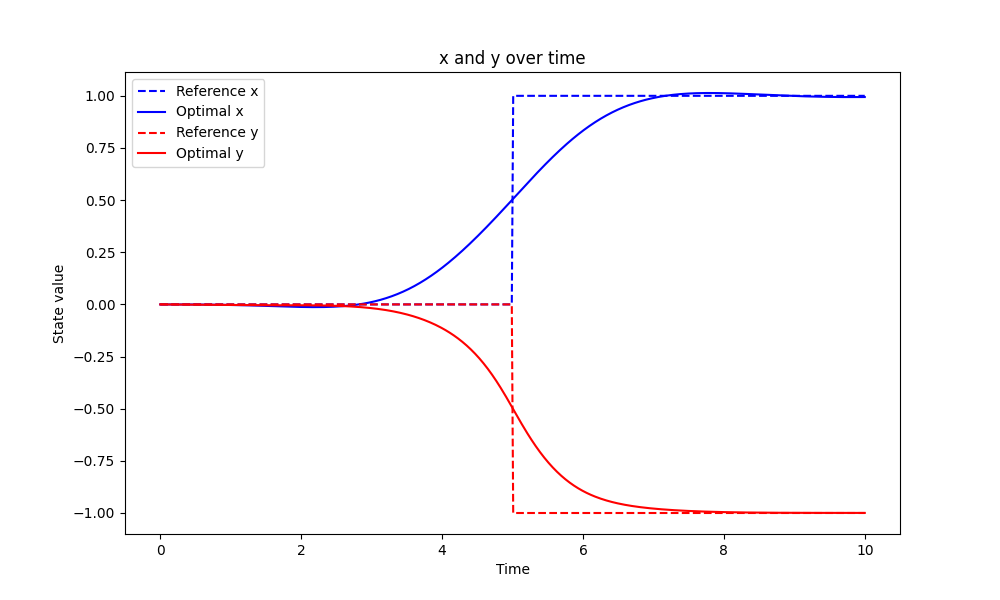
\includegraphics[width=1\textwidth]{pictures/x_y opt.png}\hfill \\
  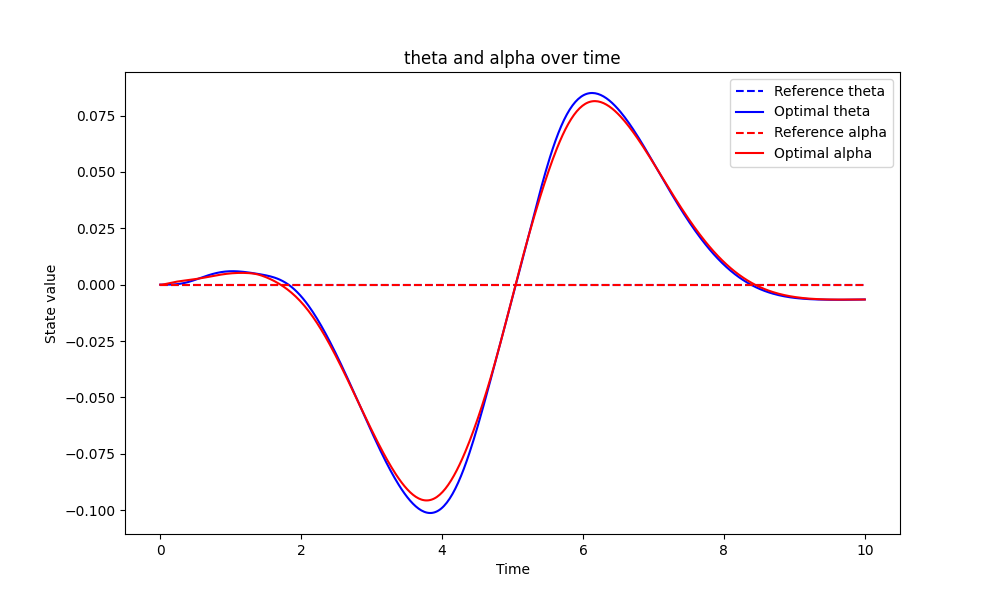
\includegraphics[width=1\textwidth]{pictures/theta alpha opt.png}\hfill
  \caption{Optimal configuration over time.}
  \label{fig:Reference trajectory}
\end{figure}

\begin{figure}[H]
  \centering
  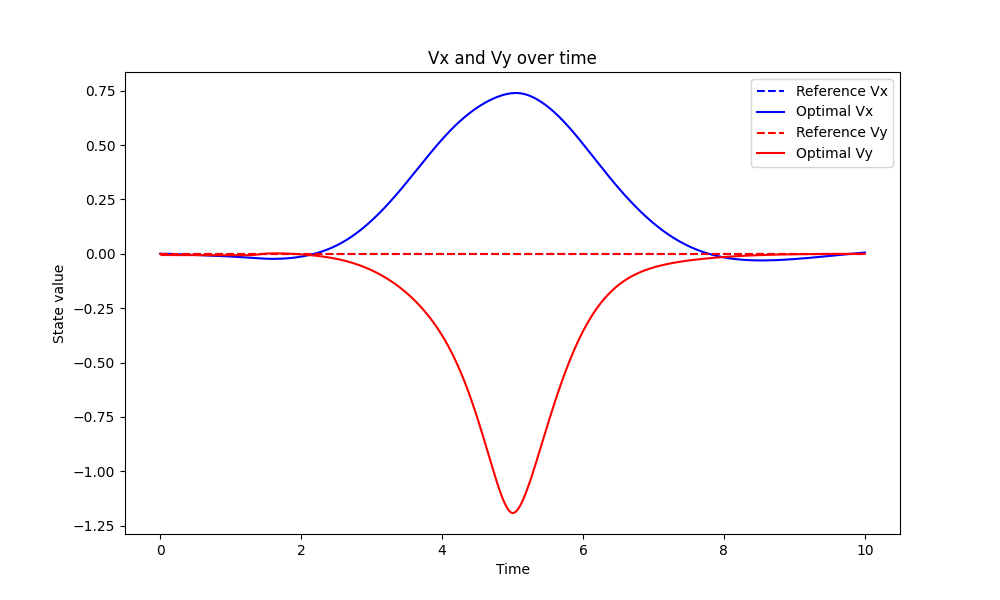
\includegraphics[width=0.85\textwidth]{pictures/vx and vy opt.png}\hfill \\
  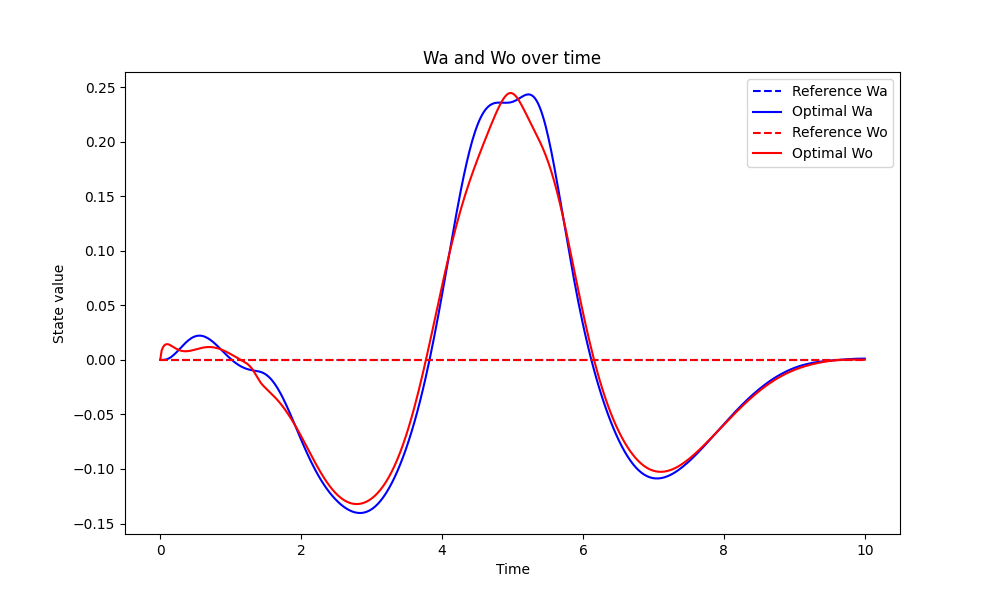
\includegraphics[width=0.85\textwidth]{pictures/omega alpha and theta.png}\hfill
  \caption{optimal velocities over time.}
  \label{fig:Reference trajectory}
  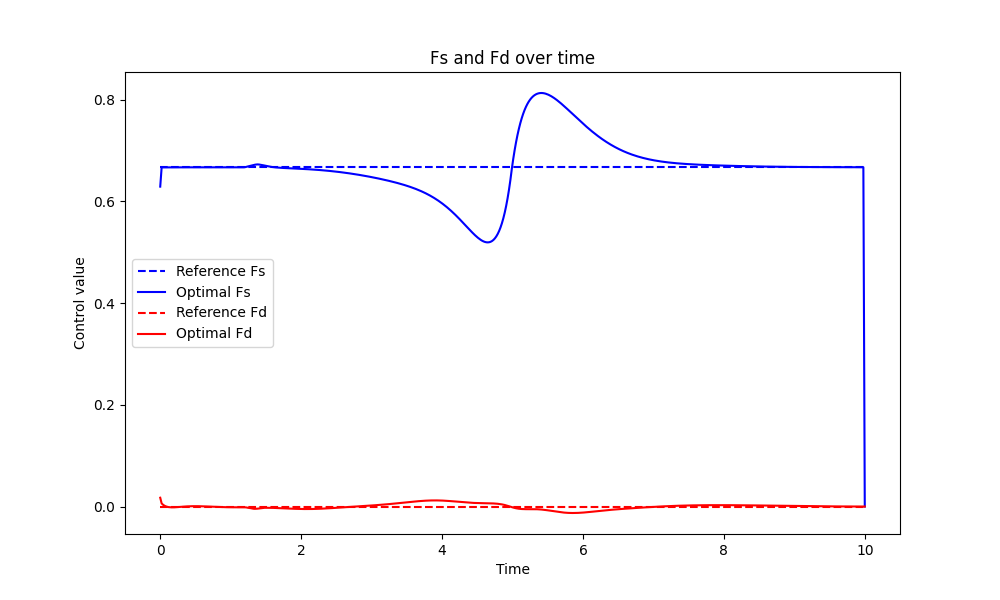
\includegraphics[width=0.85\textwidth]{pictures/Fs and Fd opt.png}
  \caption{Optimal input over time.}
  \label{fig:Reference trajectory}
\end{figure}



\subsection{Suboptimal trajectories}
To illustrate the iterative evolution of the algorithm, we display only the x and y coordinates of the quadrotor over time and the armijos plot, providing an overview of the overall progression. Refer to the code for more details.
\begin{figure}[H]
  \centering
  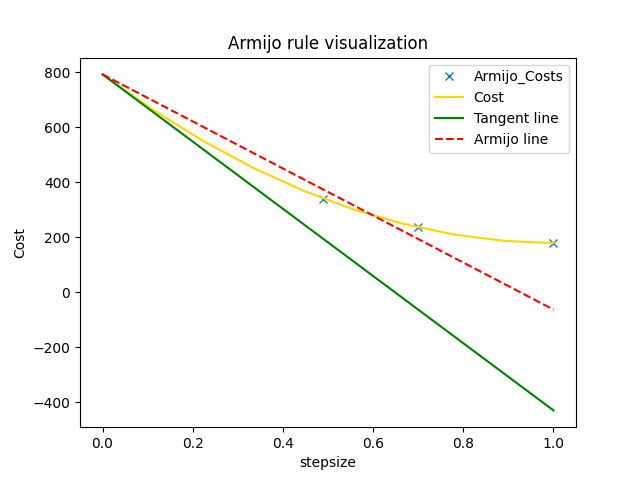
\includegraphics[width=1\textwidth]{pictures/arm_it_1.png}\hfill \\
  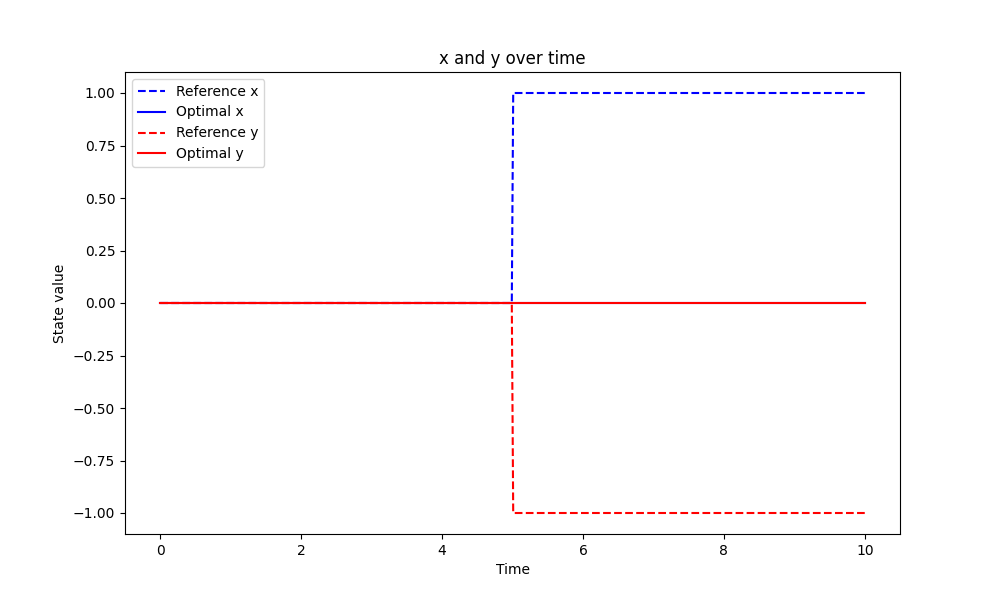
\includegraphics[width=1\textwidth]{pictures/new_it_1.png}\hfill
  \caption{First iteration.}
  \label{fig:Reference trajectory}
\end{figure}

\begin{figure}[H]
  \centering
  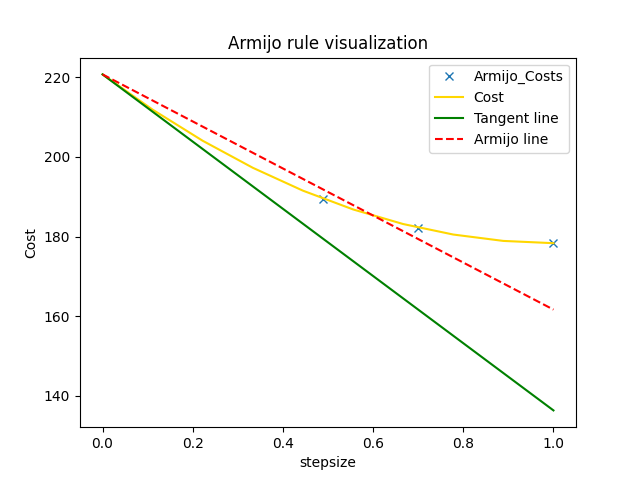
\includegraphics[width=1\textwidth]{pictures/arm_it_3.png}\hfill \\
  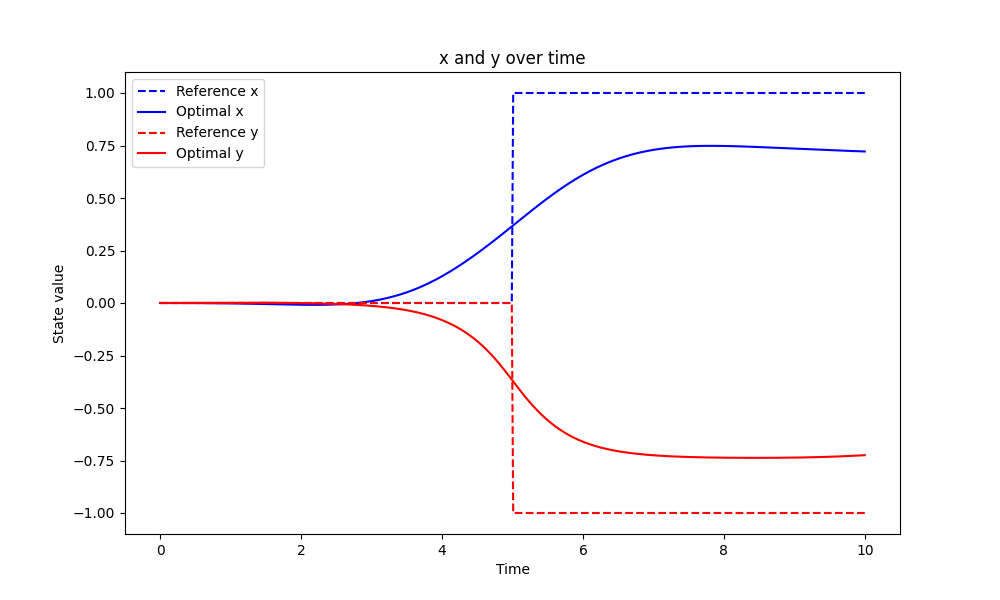
\includegraphics[width=1\textwidth]{pictures/new_it_3.png}\hfill
  \caption{Third iteration.}
  \label{fig:Reference trajectory}
\end{figure}

\begin{figure}[H]
  \centering
  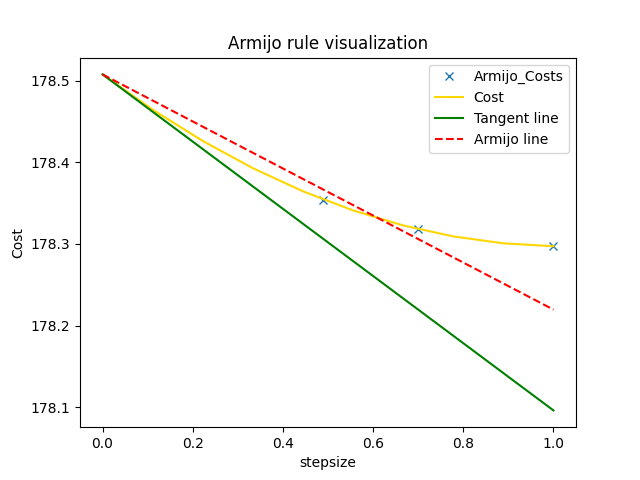
\includegraphics[width=1\textwidth]{pictures/arm_it_7.png}\hfill\\
  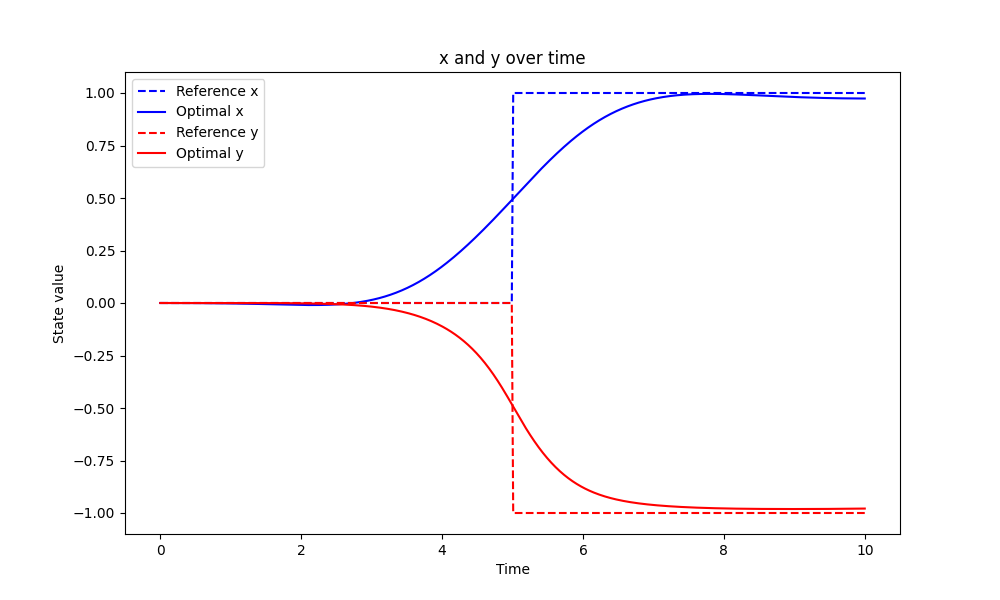
\includegraphics[width=1\textwidth]{pictures/new_it_7.png}\hfill
  \caption{Seventh iteration.}
  \label{fig:Reference trajectory}
\end{figure}

\begin{figure}[H]
  \centering
  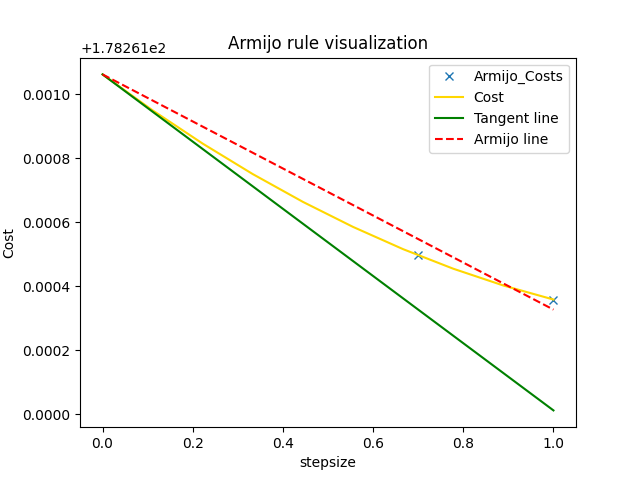
\includegraphics[width=1\textwidth]{pictures/arm_it_10.png}\hfill\\
  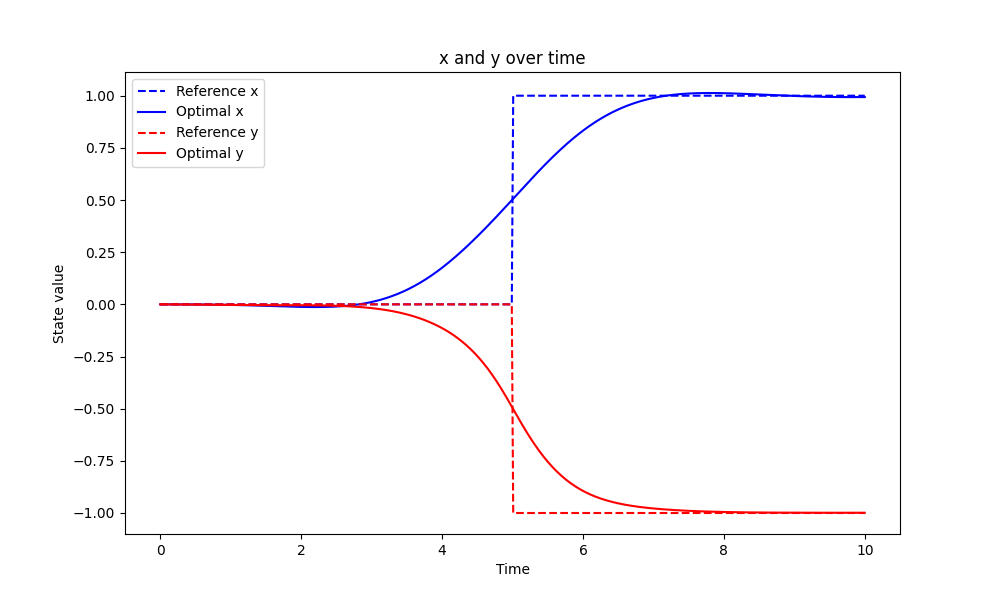
\includegraphics[width=1\textwidth]{pictures/new_it_10.png}\hfill
  \caption{Final iteration.}
\end{figure}

\subsection{Cost and Descent direction plot}
 Here the norm of the descent direction along iterations (in semi-logarithmic scale) and the cost along iterations (in semi-logarithmic scale) are shown: 
 
 \begin{figure}[h]
  \centering
  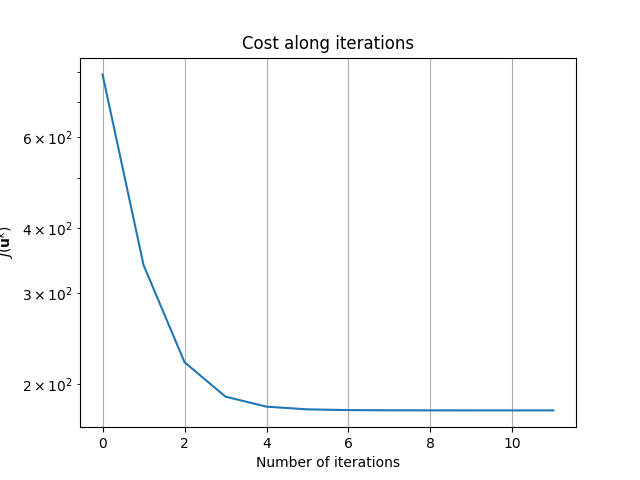
\includegraphics[width=1\textwidth]{pictures/cost_task1.png}\hfill \\
  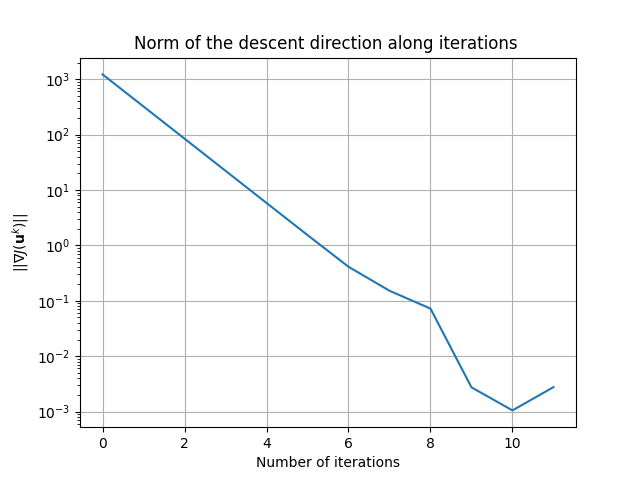
\includegraphics[width=1\textwidth]{pictures/descent_task1.png}\hfill
  \caption{Cost and descent direction norm.}
\end{figure}